\section{System Design}\label{sec:design}



Fully Sharded Data Parallel (FSDP) is capable of scaling to accommodate large models that may not fit in a single GPU device by sharding the dense parameters. More specifically, FSDP decomposes the model instance into smaller units and handles each unit independently. During forward and backward computation, FSDP only materializes unsharded parameters and gradients of one unit at a time, and otherwise, it keeps parameters and gradients sharded. Throughout the training loop, the optimizer states are kept sharded. The memory requirements for FSDP are proportional to the size of the sharded model plus the size of the largest fully-materialized FSDP unit.


\begin{figure}
    \centering
    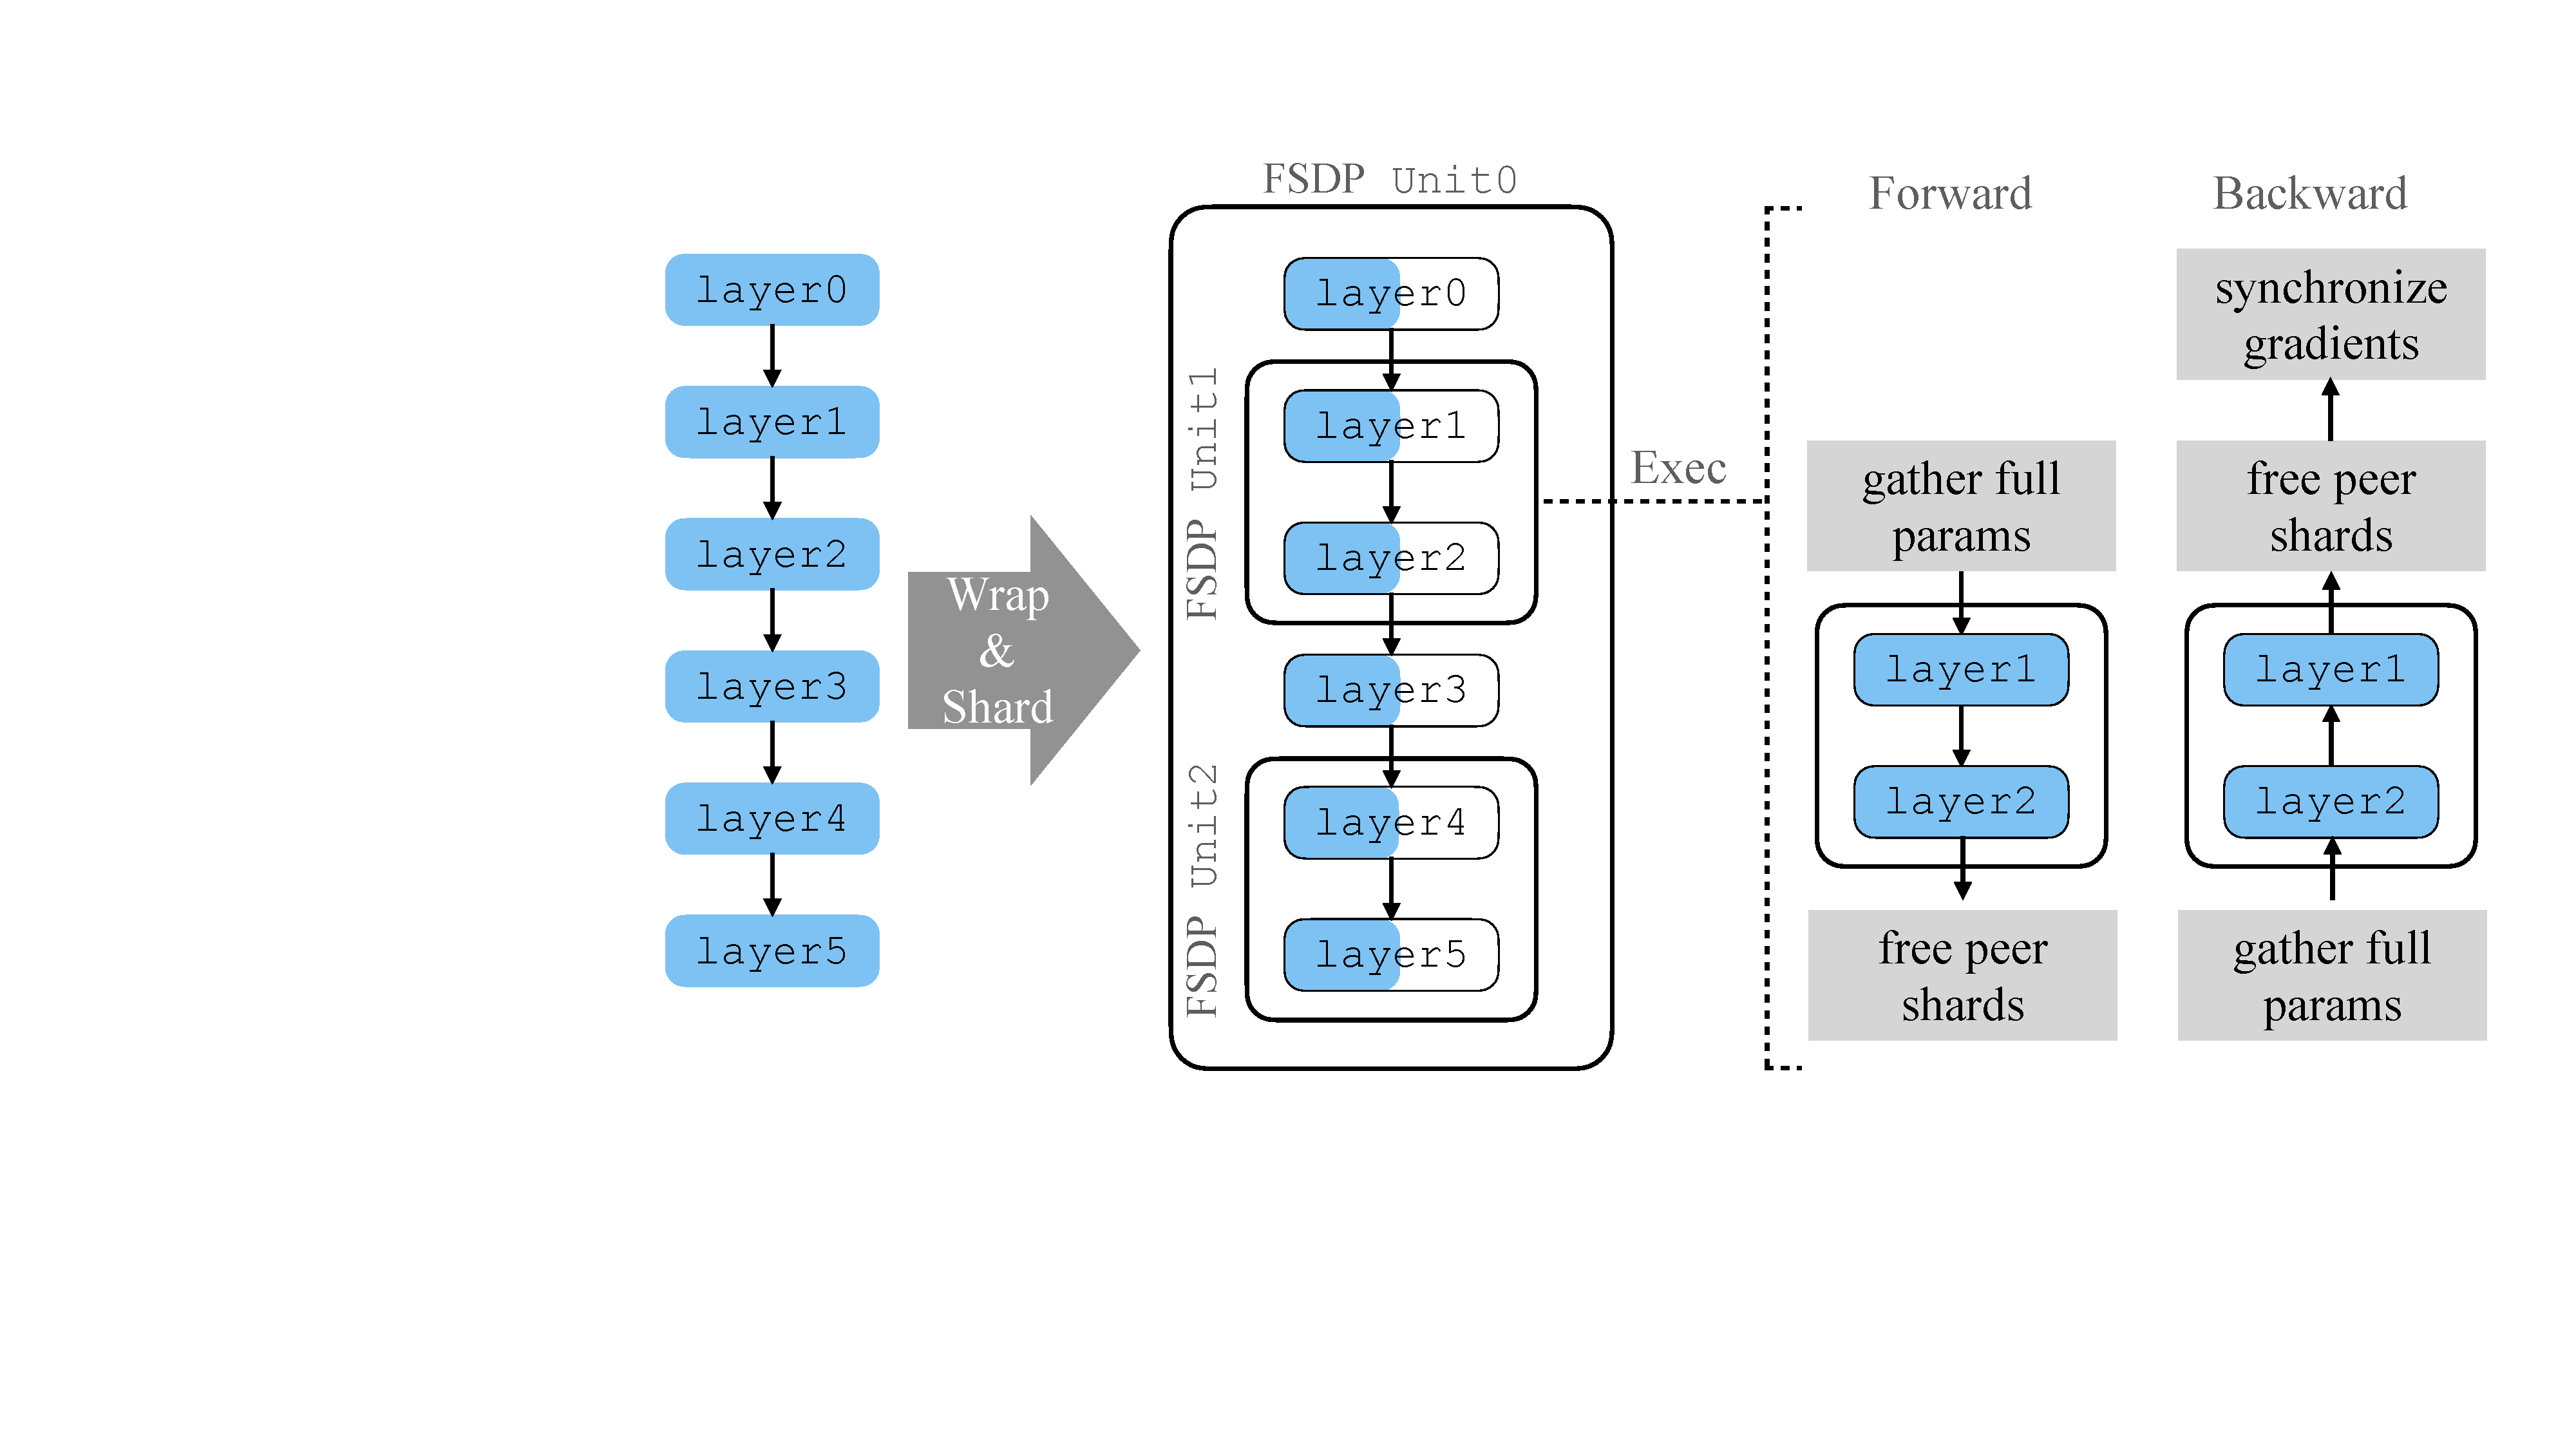
\includegraphics[width=\linewidth]{figure/overview.pdf}
    \caption{FSDP Algorithm Overview}
    \label{fig:overview}
\end{figure}

Figure~\ref{fig:overview} demonstrates the overall workflow using a simple six layer model. Suppose FSDP decomposes the model into three parts, namely, \code{[layer0, layer3]}, \code{[layer1, layer2]}, and \code{[layer4, layer5]}. The decomposition behavior can be controlled by user-defined functions. FSDP then wraps each of these three parts into one FSDP unit and shards parameters accordingly. To ensure correctness, FSDP needs to recover the unsharded parameters before corresponding computations. Let us consider FSDP \code{unit1} that contains \code{[layer1, layer2]} to explain this process. Before forward computation enters \code{layer1}, FSDP collects the unsharded parameters for \code{layer1} and \code{layer2} by gathering shards from other peer ranks. With the unsharded parameters, FSDP runs the local computation of those layers and then frees the peer shards it just collected to reduce memory footprint. Therefore, during the entire forward pass, FSDP only needs to fully materialize one unit at a time, while all other units can stay sharded. Similarly, during the backward computation, FSDP \code{unit1} recovers the unsharded parameters for \code{layer1} and \code{layer2} before backward reaches \code{layer2}. When the autograd engine finishes the backward computation of these two layers, FSDP frees the peer shards and launches \code{ReduceScatter} to reduce and shard gradients. Hence, after backward computation, each rank only keeps a shard of both parameters and gradients. 

FSDP offers a wide spectrum of optimizations and knobs to account for diverse model structures and hardware capabilities. The remainder of this section delves further into the intricacies of model initialization, sharding strategies, communication optimizations, and memory management, which are all critical components of FSDP's underlying design.


\subsection{Model Initialization}

Before the advent of FSDP, PyTorch mandated the full materialization of the entire model instance on one device. Although users can allocate different sub-modules to different devices, this would require modifying the model source code, which may not be feasible, particularly if model authors and application developers belong to different parties. To facilitate a smooth transition from local to distributed training, FSDP must effectively aid in the materialization and initialization of a massive model, which poses two challenges:

\begin{itemize}
    \item How to create a model instance without materializing any tensor storage, postponing initialization until a storage on a concrete device is attached to the tensor.
    \item How to ensure accurate initialization of model parameters in line with the user's implementation, even when the model is too large to fit on a single GPU. 
\end{itemize}

To overcome the first challenge, we have introduced a mechanism called \emph{deferred initialization}, which involves the allocation of model parameter tensors on a simulated or "fake" device. During this process, all initialization operations performed on the tensor are recorded. Subsequently, when the tensor is moved from the "fake" device to a GPU device, all recorded operations are automatically replayed. By adopting this technique, users can generate a model instance from any third-party library without allocating any GPU memory blocks, while still accurately capturing their parameter initialization implementations.

As illustrated in Figure~\ref{fig:overview}, once the FSDP has wrapped the model, it is evenly distributed across all GPUs, with each device holding only one shard in its memory. Therefore, in order to address the second challenge, each rank should ideally only materialize and initialize the shard that it owns. However, this is not always practical, since we cannot predict what initialization logic the user will implement in the model \code{init} method. The initialization logic may rely on having a unsharded parameter on the device, which makes it impossible to shard the initialization. Consequently, FSDP must prepare the unsharded parameters before executing \code{Tensor} initialization operations and simultaneously reduce the memory footprint. Given that sharding initialization is unsafe, FSDP applies the same approach as how it handles model forward and backward passes, \emph{i.e.}, initialize one FSDP unit at a time and shard the unit before moving on to the next one. When combined with deferred initialization, FSDP traverses the fake device model instance to decompose it into FSDP units, moves one unit to a GPU device at a time, and replays the recorded initialization operations for tensors in that FSDP unit.



%%%%%%%%%%%%%




\subsection{Sharding Strategies}\label{sec:sharding_strategy}

The \emph{sharding strategy} is an important element in FSDP that plays a significant role in determining the memory footprint and communication overhead.  FSDP offers a variety of sharding strategies, ranging from fully replicated to fully sharded. To generalize these sharding strategies, we introduce the \textit{sharding factor} $F$ as the number of ranks over which parameters are sharded. By setting the sharding factor to $1$, FSDP fully replicates the model and simplifies to vanilla data parallelism that uses \code{AllReduce} for gradient reduction. By setting the sharding factor equal to the number of devices (\emph{i.e.}, global world size $W$), FSDP fully shards the model, with each device only holding $\frac{1}{W}$ of the model. Hybrid sharding occurs when the sharding factor ranges between $1$ and $W$. The remainder of this section focuses on full sharding and hybrid sharding since the full replication strategy is similar to the existing DDP~\cite{ddp}.

\subsubsection{Full Sharding}\label{sec:full_shard}\hfill \break

The \emph{full sharding} strategy leads to the lowest memory footprint but incurs the most communication overhead, for example, \emph{full sharding} has 1.5x communication overhead and volume over DDP if using bandwidth optimal ring algorithm. Therefore, FSDP must carefully organize communications to maximize its efficiency under this strategy.

\begin{figure}

\begin{minipage}[c]{0.22\textwidth}
  \centering
  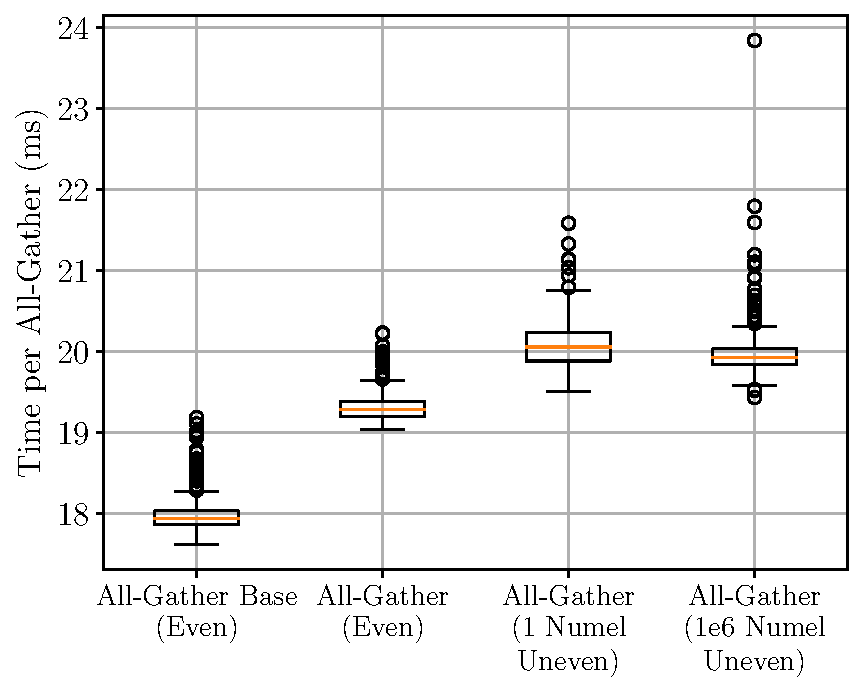
\includegraphics[width=\linewidth]{figure/time_per_all_gather_vs_config.pdf}
  (a) Uneven Input Sizes
\end{minipage}
\begin{minipage}[c]{0.235\textwidth}
  \centering
  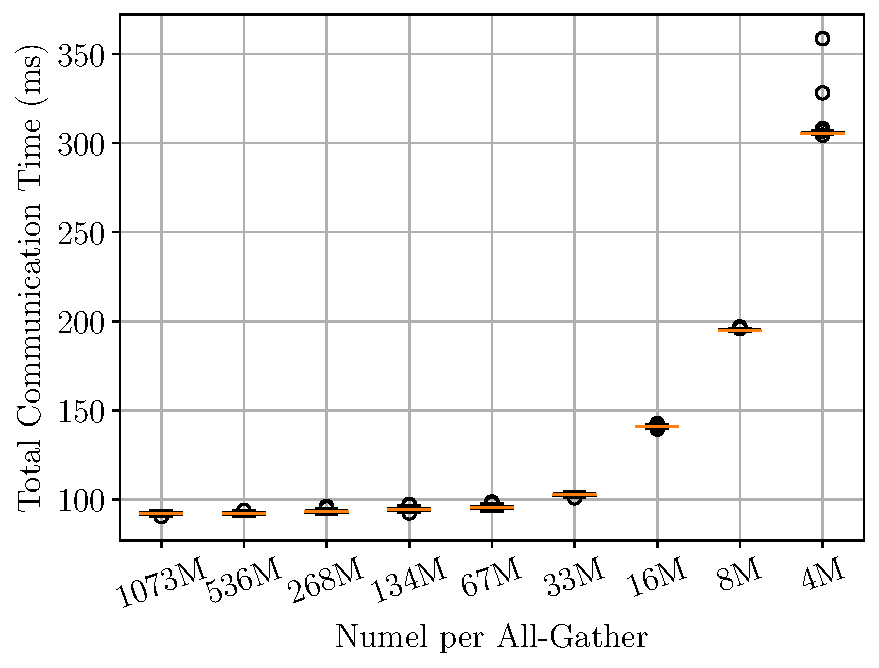
\includegraphics[width=\linewidth]{figure/time_vs_input_size.pdf}
  (b) Reducing Input Size
\end{minipage}
\caption{Communication Efficiency vs. Input Size}\label{fig:comm_evidence}
\end{figure}


We conducted two sets of experiments to understand the impact of input size on collective communication efficiency. Results are shown in Figure~\ref{fig:comm_evidence}, which helped identify two ingredients for efficiencies:
\begin{enumerate}
    \item \textbf{Even Input Size:} The Nvidia NCCL~\cite{nccl} library offers efficient collective implementations for all-gather and reduce-scatter that require \emph{even} input tensor sizes across ranks.
    \item \textbf{Larger Input Size:} For fixed communication volume, batching data and issuing fewer collectives improves performance by avoiding the collectives' launch overhead and increasing network bandwidth utilization.
\end{enumerate}

For (1), NCCL's \code{AllGather} API requires even input tensor size and writes outputs into one single tensor. PyTorch's \code{ProcessGroup} wraps the NCCL API and enhances it by supporting uneven input tensor sizes across ranks and allowing users to provide a list of output tensors. The flexibility comes with an efficiency trade-off, as shown in Figure~\ref{fig:comm_evidence}~(a). We use \code{All-Gather Base} to denote NCCL's \code{AllGather} behavior, and \code{All-Gather} to denote the one that takes a list of tensors as outputs. The latter incurs additional copies between the individual output tensors and the consolidated single large output tensor before and after the communication. Moreover, for uneven inputs, \code{ProcessGroup} mimics \code{AllGather}'s behavior using group \code{Broadcast}, which is slower than \code{All-Gather Base}. In the experiments, we created artificial unevenness by moving $1$ element and $1e6$ elements from rank 1 to rank 0 respectively. The results show that the \code{All-Gather Base} with even input size achieved highest efficiency. 

For (2), Figure~\ref{fig:comm_evidence}~(b) fixes the total communication to be $2^{30} \approx 1\text{B}$ \code{FP32} elements and varies the size per \code{All-Gather}, \emph{i.e.}, smaller \code{AllGather} size means more \code{AllGather} invocations. Once the \code{AllGather} size decreases below $33\text{M}$ elements, the total communication time begins increasing rapidly.

Thus, to deliver highly efficient communications, FSDP organizes all parameters within one FSDP unit into a large \code{FlatParameter}, where the \code{FlatParameter} coalesces the communications of its individual parameters and also evenly shards them across ranks. More specifically, the \code{FlatParameter} is a 1D tensor constructed by concatenating $p$ flattened original parameters and padding on the right to achieve a size divisible by the sharding factor. To shard the \code{FlatParameter}, FSDP divides it into equal-sized chunks, where the number of chunks equals the sharding factor, and assigns one chunk per rank. The \code{FlatParameter}'s gradient inherits the same unsharded and sharded shapes from the \code{FlatParameter}, and the \code{FlatParameter} and its gradient own the underlying storage of the original parameters and their gradients, respectively. Figure~\ref{fig:full_sharding} depicts one example, where we use one FSDP unit to shard a $4\times 3$ \code{nn.Linear} layer across 16 GPUs. In this case, every GPU only holds one element from the \code{FlatParameter} with the last rank holding the padded value. 

\begin{figure}
    \centering
    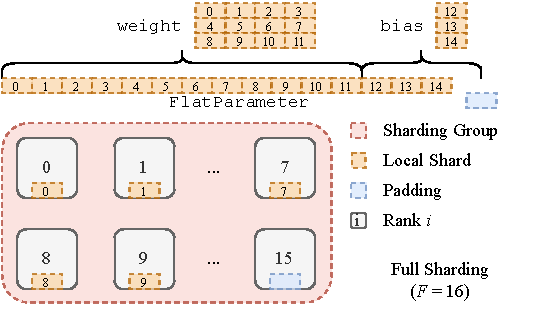
\includegraphics[width=\linewidth]{figure/full_sharding.pdf}
    \caption{Full Sharding Across 16 GPUs}
    \label{fig:full_sharding}
\end{figure}

This flatten-concat-chunk algorithm permits each original parameter to have arbitrary shape while minimizing the required padding (to be at most $F-1$), reflecting its generality. 
%However, the does come at the cost of structure: An original parameter may be split across ranks such that it cannot be reshaped to a sharded version of its original shape. Regardless, 
Moreover, under this algorithm, the sharded and unsharded \code{FlatParameter} and its gradient have the exact data layout expected by \code{AllGather} and \code{ReduceScatter}, respectively. This enables calling the collectives without any additional copies for either the input or output tensors.
% Thus, the \code{FlatParameter} and its gradient represent the atoms for FSDP's collectives.

More formally, suppose for a model with $\Psi$ number of elements, FSDP constructs $N$ \code{FlatParameter}s with numels $\psi_1, \dots, \psi_N$, where $\sum_{i=1}^N \psi = \Psi$. For sharding factor $F$, the peak parameter memory contribution is in $O(\sum_{i=1}^N \frac{\psi_i}{F} + \max_{i=1}^N \psi_i)$ because FSDP always keeps each local sharded \code{FlatParameter} with size $\frac{\psi_i}{F}$ in GPU memory and must materialize each unsharded \code{FlatParameter} with size $\psi_i$ one by one during forward and backward. Since the first $\sum_{i=1}^N \psi_i = \Psi$ is fixed, the peak parameter memory contribution is determined by $\max_{i=1}^N \psi_i$. At the same time, the number of collectives per iteration is in $O(N)$. This evidences FSDP's memory-throughput trade-off: Finer-grained \code{FlatParameter} construction decreases peak memory but may decrease throughput by requiring more collectives. Users can control this trade-off by specifying how to wrap sub-modules into FSDP units.

\subsubsection{Hybrid Sharding}\hfill \break

We refer to the strategy when the sharding factor is greater than $1$ but less than $W$ as \textit{hybrid sharding}, as it combines both sharding and replication. For global world size $W$ and sharding factor $F$, the parameters are sharded within each group $S_1, \dots, S_{W/F}$ and are replicated within each complementary group $R_1, \dots, R_F$, where each $S_i, R_j \subseteq \{1, \dots, W\}$ gives the ranks in the sharded or replicated group, respectively.

\begin{figure}
    \centering
    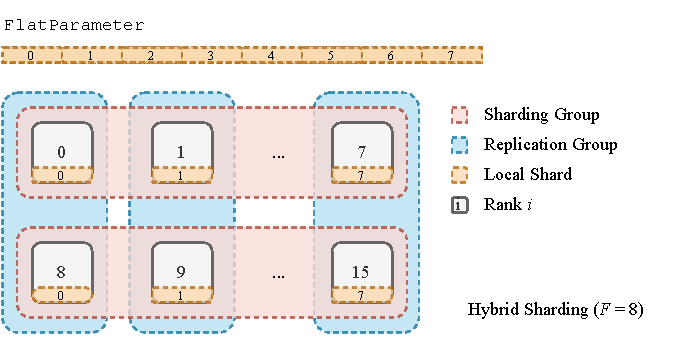
\includegraphics[width=\linewidth]{figure/hybrid_sharding.pdf}
    \caption{Hybrid Sharding on 16 GPUs: GPUs are configured into 2 sharding groups and 8 replication groups}
    \label{fig:hybrid_sharding}
\end{figure}

For gradient reduction, the single reduce-scatter over all ranks becomes a reduce-scatter within each of the sharded groups followed by an all-reduce within each of the replicated groups to reduce the sharded gradients. The equivalence follows from the decomposition
\begin{equation}
    \sum_{r=1}^W g_r = \sum_{i=1}^{W/F} \sum_{r \in S_i} g_r,
\end{equation}
where $g_r$ represents the gradient on rank $r$.

% \todo[inline]{Figure showing equivalence of global RS and RS + AR}

Hybrid sharding can take advantage of datacenter locality for accelerated training and can reduce cross host traffic to avoid as much contention in the oversubscribed environment as possible. At the same time, it provides a graduating trade-off between memory saving and throughput degradation, which is particularly helpful for models whose required memory footprint when trained with full replication is just slightly above the device capacity and do not want full sharding. Figure~\ref{fig:hybrid_sharding} shows one example. 

Specifically, datacenters typically adopt a fat-tree network topology~\cite{liu2017incbricks} with over-subscription, leading to abundant locality to exploit and a well-motivated reason to reduce cross-host traffic~\cite{luo2020plink}. Hybrid sharding can provide a natural mechanism to map the device mesh into the datacenter layout to exploit such locality. For example, consider a cluster as a group of $W$ accelerators grouped into hosts of of $G$ accelerators each (where the communication among accelerators on the same host is much faster than the communication across hosts), we can set $F = \frac{W}{G}$ to limit the \code{AllGather} (and \code{ReduceScatter}) operations within the same host, while creating a replication group for accelerators with the same local rank across hosts. For an $M$-sized model, we can then compute the total cross-host traffic per GPU in the hybrid setup to be $2M\frac{W-1}{GW}$, a drastic reduction compared to full replication's $2M\frac{W-1}{W}$ and full sharding's $3M\frac{W-1}{W}$. Additionally, since the \code{AllReduce} collectives used in hybrid sharding operates at a smaller world size, they empirically achieve a better performance than invoking collectives at the global scale (in the case of full replication and full sharding), due to straggler effects and larger network interference. 

Another important design motivation for hybrid sharding is the needs from medium-sized models. These models are large enough to cause out of memory issues when trained with full replication but are not large enough to fully utilize accelerator memory when used with full sharding, leading to \emph{both} runtime overhead and memory waste. The hybrid sharding strategy creates a much richer memory-throughput trade-off space by simply adjusting $F$.

% We highlight one particular case of hybrid sharding that is performant for medium-sized models. For context, communication backbones in modern datacenter components are both hierarchical and heterogeneous. The fat-tree topology~\cite{liu2017incbricks} with different link speeds at different levels and over-subscription naturally lead to abundant locality to exploit. Failure to tap into this property often results in subpar scalability and performance~\cite{luo2020plink}. In particular, clusters are typically organized as a group of nodes with each node consisting of a group of accelerators, where the communication is faster intra-node and slower intra-node. Thus, to exploit this heterogeneity, a performant choice of sharding factor is the intra-node size (\textit{e.g.}\ 8 for typical Nvidia GPU nodes), meaning that parameters are only sharded within each node. This changes the global reduce-scatter to an intra-node reduce-scatter followed by an inter-node all-reduce.

\subsubsection{Autograd}
\label{subsubsection:autograd}\hfill \break

FSDP's \code{FlatParameter} must inter-operate with PyTorch's autograd engine to ensure (1) correct gradient propagation and (2) timely gradient reduction. For (1), recall that the \code{FlatParameter} and its gradient own the underlying storage of the original parameters and their gradients, respectively. To achieve this, before forward computation, FSDP sets the original parameters to be views into their unsharded \code{FlatParameter} using \textit{autograd-visible} \code{torch.split()} and \code{torch.view()} calls. Then, the autograd engine naturally allocates the unsharded \code{FlatParameter} gradient and writes each original parameter's gradient to the appropriate offset as defined by \code{torch.split()}'s backward function. For (2), FSDP registers a gradient hook that only runs once the \code{FlatParameter}'s gradient is finalized. The hook represents the post-backward logic and includes the gradient reduction. Notably, FSDP's approach builds on top of PyTorch's autograd engine instead of hacking around it. As a result, FSDP automatically handles unconventional cases such as when not all parameters are used in the forward or when there are multiple forwards before a backward.

%%%%%%%%%%%%%%

%This section describes FSDP's different variations, termed as \textit{sharding strategies}, and their runtime schedules.

%\subsubsection{Preliminaries}
%During computation, a parameter must be unsharded, and only outside of computation can it be resharded. To characterize FSDP's runtime schedule, we define per-parameter \code{unshard} and \code{reshard} operations. \code{unshard} involves allocating memory, running all-gather, and switching the parameter from sharded to unsharded data, and \code{reshard} involves switching the parameter from unsharded to sharded data and freeing memory.

%Moreover, for a given training iteration and each parameter we can define \textit{pre/post-forward/backward} to be right before/after the parameter's forward/backward computation, respectively. FSDP may choose to insert its own logic at these four points. For example, gradient reduction happens in the post-backward.

% for the model, we can further define the \textit{prologue} to proceed the entire forward and the \textit{epilogue} to follow the entire backward.
% To-do: Maybe we do not need to define prologue and epilogue here

%\subsubsection{Sharding Strategy Space}
%\label{subsubsection:sharding_strategy_space}
%FSDP offers two main variations on the unshard/reshard schedule for each parameter:
%\begin{itemize}
%   \item Reshard after forward: pre-forward \code{unshard}, post-forward \code{reshard}, pre-backward \code{unshard}, post-backward \code{reshard}
%   \item No reshard after forward: pre-forward \code{unshard}, post-backward \code{reshard}
%\end{itemize}
%\todo[inline]{Decide how we want to name/refer to above}

%In other words, with resharding after forward, each parameter is only unsharded for its forward and backward computations and is resharded immediately outside of that. In contrast, without resharding after forward, after a parameter is unsharded during forward, it remains unsharded through the rest of forward and through backward until after its gradient computation. This increases peak memory but saves one all-gather per parameter.

%We define the \textit{sharding factor} to be the number of ranks over which parameters are sharded. In addition to the unshard/reshard schedule, we may additionally parameterize over the sharding factor, allowing it to be any integer factor of the global world size. Together, these define the sharding strategy space through which FSDP offers a unified data parallel solution.

%By setting the sharding factor to one, FSDP simplifies to vanilla data parallelism without sharding and uses all-reduce for gradient reduction. By setting the sharding factor equal to the global world size and resharding after forward, FSDP implements ZeRO-3; by not resharding after forward, FSDP achieves the same model-state peak memory contribution as ZeRO-2~\cite{zero}. These use reduce-scatter for gradient reduction.

%\subsubsection{Hybrid Sharding}




\subsection{Communication Optimizations}

The FSDP framework incorporates a range of native communication optimization techniques. This section unveils four major ones: overlapping, backward pre-fetching, forward pre-fetching, and accumulation. 

\subsubsection{Overlapping Communication and Computation} \hfill \break

The PyTorch \code{c10d} library has a \code{ProcessGroup} abstraction that represents a group of processes that can run collectives together. For the NCCL backend, the \code{ProcessGroupNCCL} implementation has an internal NCCL stream per device, where the separate internal stream is for asynchronous execution with the current stream, which is typically the default stream running computation. Those asynchronous collectives return \code{Work} objects, where calling \code{Work.wait()} blocks the CPU thread until the collective finishes. For general correctness, \code{ProcessGroupNCCL} synchronizes the internal stream with the current stream before running the collective. \code{DistributedDataParallel} leverages the async-collective-and-\code{wait()} approach to overlap the gradient \code{All-Reduce}s with backward computation. However, in contrast to DDP's backward where the \code{AllReduce} \textit{proceeds} the computation with which to overlap, FSDP's forward issues the \code{AllGather} \textit{following} the computation with which to overlap since in eager execution, FSDP cannot know which \code{FlatParameter} to \code{AllGather} next to reorder it before the computation. This difference in kernel-issue order makes following the async-collective-and-\code{wait()} approach infeasible for FSDP. Namely, since \code{ProcessGroupNCCL} synchronizes with the current (default) stream, the \code{All-Gather} will not run until the computation with which to overlap finishes. To address this, FSDP uses a separate CUDA stream to issue the \code{AllGather}s, bypassing the false dependency on preceding computation in the default stream and allowing each \code{AllGather} to overlap. As a result, FSDP's collective synchronization operates on streams, not simply \code{Work} objects. Figure~\ref{fig:overlap} illustrates one example. Note that the backward pass excludes the \code{AG0} \code{All-Gather} because FSDP intentionally keeps the outermost FSDP unit's parameters in memory to avoid redundantly freeing at the end of forward and then re-\code{All-Gather}ing to begin backward.

% As a side optimization, both the \code{ReduceScatter} and \code{AllReduce} (when hybrid shard is on) can run asynchronously with respect to the backward pass, as they are not needed until the optimizer step.

\begin{figure}
    \centering
    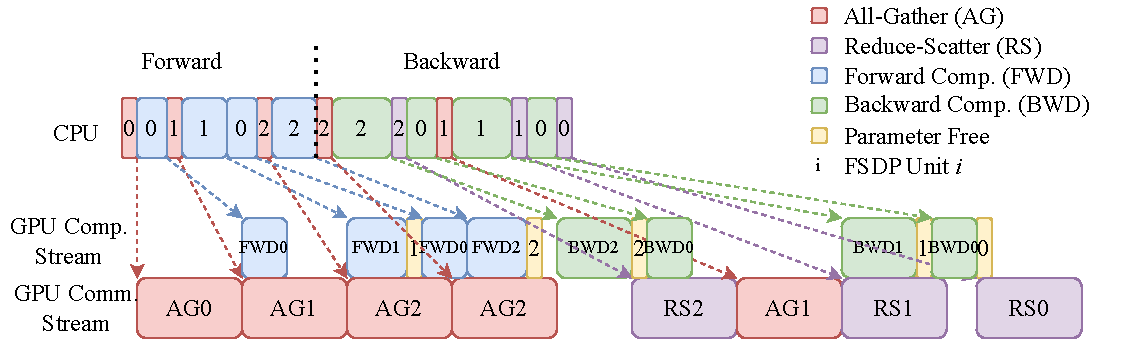
\includegraphics[width=\linewidth]{figure/overlap.pdf}
    \caption{Overlap Communication and Computation}
    \label{fig:overlap}
\end{figure}

\subsubsection{Backward Prefetching} \hfill \break

FSDP enforces a single CUDA device per rank and uses a single process group for both \code{AllGather} and \code{ReduceScatter}, which means that its collectives run sequentially in the process group's internal NCCL stream. In the backward pass, FSDP issues the \code{ReduceScatter} for the current \code{FlatParameter} and then the \code{AllGather} for the next \code{FlatParameter}. Hence, the single NCCL stream forces the \code{ReduceScatter} to block the next \code{AllGather}, which in turn blocks the next gradient computation and may become exposed on the critical path.

To avoid two consecutive exposed communication calls in the backward pass, FSDP \textit{backward prefetching} issues the next \code{AllGather} before the current \code{ReduceScatter}. However, as mentioned before, a challenge for eager execution is knowing which \code{FlatParameter} to \code{AllGather} next. FSDP resolved this challenge by recording the reverse forward execution order of modules as the proxy of their backward execution order. Moreover, the forward order is freshly recorded each iteration, meaning that the \textit{backward prefetching} is compatible with dynamism across iterations.

%\todo[inline]{Backward prefetching figure: reorder RS and AG}

\subsubsection{Forward Prefetching} \hfill \break

For some workloads with relatively slow CPU execution, the CPU thread may not be able to issue the next forward \code{AllGather} early enough to efficiently fill the NCCL stream. If the model follows a static computational graph across iterations, then FSDP can assume the forward execution order of modules from the previous iteration and prefetch the next \code{AllGather} explicitly in the forward pass. This \textit{forward prefetching} issues the next \code{AllGather} before forward computation of current FSDP unit.


\subsubsection{Gradient Accumulation} \hfill \break

FSDP offers two variations of gradient accumulation: with and without communication. With communication, FSDP still reduces gradients across ranks, and each rank saves the sharded gradients. Simply running multiple iterations without clearing gradients achieves this. Without communication, FSDP does not reduce gradients across ranks, and each rank saves the unsharded gradients. This latter variation trades off increased memory usage with decreased communication, which can increase end-to-end throughput.


\subsection{Memory Management}\label{sec:memory_management}

%\subsubsection{Rate Limiter} \hfill \break
PyTorch uses a CUDA caching allocator as a middle layer to serve GPU allocation and free requests for PyTorch programs. In order to effectively manage memory, FSDP uses a \textit{rate limiter} to take into account the memory impact of the caching allocator on programs that use several CUDA streams and run fast CPU threads.

\subsubsection{How Does PyTorch Caching Allocator Affect Memory}
\label{subsubsection:pytorch caching allocator}\hfill \break

The caching allocator avoids frequent calls to \code{cudaMalloc} and \code{cudaFree}, where the latter incurs a costly device synchronization. Specifically, the caching allocator requests CUDA memory blocks and internally determines how to split and reuse the blocks without returning them to CUDA with the goal being to reach a steady state without further calls to \code{cudaMalloc} and \code{cudaFree}.

The caching allocator runs from the CPU thread, meaning that it must decide which caching allocator block to use for an allocation when the \textit{CPU thread} processes the allocation request. It cannot wait until the GPU kernel needing the allocation actually runs, which may be much later. 

For a single stream, the caching allocator can directly reuse memory blocks by the stream's sequential ordering semantics. However, for separate producer and consumer streams, there are no inter-stream ordering guarantees, and the caching allocator cannot be certain that a block is safe to reuse until the last \textit{GPU kernel} depending on that memory finishes running. Hence, if the CPU thread runs far ahead of the GPU execution, then the caching allocator cannot reuse blocks for the producer stream with pending GPU kernels from the consumer stream.

Furthermore, caching allocator blocks are allocated \textit{per stream} and cannot be reused for a different stream, this over-allocates blocks to the producer stream that could otherwise be used for the consumer stream (\textit{e.g.}\ for activations). The GPU itself may have enough memory to serve a new allocation in the consumer stream, but the overallocation to the producer stream may lead to the caching allocator failing to serve it. This forces a blocking sequence of \code{cudaFree}s to reset the caching allocator memory state called a \code{cudaMalloc} retry that greatly degrades training throughput.

\subsubsection{Rate Limiter}
\label{subsubsection:rate limiter}\hfill \break

FSDP allocates the \code{AllGather} destination tensor representing the unsharded \code{FlatParameter} in a producer stream, and the forward and backward computations using the \code{AllGather}ed parameters run in a consumer stream (typically the default stream). For a fast CPU thread, there may be pending GPU computation kernels when the caching allocator must serve the next \code{AllGather}, leading to no block reuse. Even after the blocks are not active in the \code{AllGather} producer stream, these reserved blocks can not serve default computation stream's allocation requests, and thus may force blocking \code{cudaFree}s and \code{cudaMalloc}s. 

%\todo[inline]{Add figures showing that CPU allocation must be served after previous GPU computation to reuse the block}

FSDP offers a \textit{rate limiter} that intentionally blocks the CPU thread to ensure proper caching allocator block reuse. It allows at most two inflight \code{AllGather}s, which is the minimum amount to still achieve communication and computation overlap.

